\documentclass[sigconf,anonymous]{acmart}
\usepackage{amsmath}
\usepackage{booktabs}
\usepackage{tabularx}
\usepackage{balance}
\usepackage{siunitx}
\sisetup{group-minimum-digits=4,group-separator={,}}
\settopmatter{printacmref=false,printfolios=true,printccs=false}
\setlength{\emergencystretch}{1.5em}
\vfuzz=2pt
\setcopyright{none}
\renewcommand\footnotetextcopyrightpermission[1]{}
\acmConference[SIGMOD 2027]{SIGMOD 2027}{Under review}{Anonymous submission}
\acmBooktitle{SIGMOD 2027 Experiments \& Analysis submission}
\acmYear{2027}
\copyrightyear{2027}
\acmDOI{}
\acmISBN{}
\newcommand{\risk}{\mathcal{R}}
\newcommand{\ndc}{\operatorname{NDC}}
\newcommand{\rec}{\operatorname{Recall}}
\newcommand{\indicator}{\mathbf{1}}
\newcommand{\slot}[2]{%
  \fbox{\parbox{\dimexpr\linewidth-2\fboxsep-2\fboxrule\relax}{%
  \small\textbf{Planned exhibit: #1}\par\medskip #2}}}
\newcommand{\sectionaim}[1]{\noindent\textit{Section purpose: #1}\par}

\newcommand{\GraphOnlyRows}{%
hnswlib HNSW & SIFT & 22.31 & 0.77 & 21.55 [20.76, 22.33] & 89.33 \\
Faiss HNSW & SIFT & 23.67 & 0.07 & 23.60 [22.78, 24.39] & 91.07 \\
hnswlib HNSW & Arxiv & 18.24 & 1.07 & 17.17 [16.33, 18.06] & 75.87 \\
Faiss HNSW & Arxiv & 17.93 & 0.17 & 17.77 [16.86, 18.68] & 75.87 \\
}
\newcommand{\RecoveryRows}{%
SIFT & Endpoint & 0.97 [0.53, 1.50] & 0.00 [0.00, 0.00] & 1,826 & 2,615 & 2,855 \\
SIFT & Direct reuse & 6.69 [5.65, 7.77] & 59.51 [57.83, 61.20] & 739 & 2,132 & 2,706 \\
SIFT & Original recalibration & 1.79 [1.25, 2.40] & 44.39 [42.76, 46.01] & 1,015 & 2,349 & 2,774 \\
SIFT & Joint-error replay & 1.79 [1.25, 2.40] & 44.39 [42.76, 46.01] & 1,015 & 2,349 & 2,774 \\
\addlinespace
Arxiv & Endpoint & 1.01 [0.61, 1.47] & 0.00 [0.00, 0.00] & 2,397 & 3,252 & 3,504 \\
Arxiv & Direct reuse & 7.24 [6.18, 8.36] & 64.21 [62.51, 65.85] & 858 & 2,586 & 3,322 \\
Arxiv & Original recalibration & 2.04 [1.45, 2.69] & 44.79 [34.32, 50.96] & 1,323 & 2,974 & 3,398 \\
Arxiv & Joint-error replay & 1.68 [1.10, 2.35] & 29.86 [14.75, 45.00] & 1,681 & 3,117 & 3,460 \\
\addlinespace
}
\newcommand{\CostRows}{%
SIFT & Cached & 129 [129, 129] & 0/10 \\
SIFT & Cold & 396 [395, 397] & 0/10 \\
Arxiv & Cached & 148 [99, 296] & 4/10 \\
Arxiv & Cold & 457 [305, 915] & 4/10 \\
}
\newcommand{\CertificateRows}{%
S & 1103 & 1 & 9 & 3.12 & 3.39 & 2 & 1.44 & C & 1.50 & 44.33 \\
S & 1229 & 1 & 8 & 2.87 & 3.13 & 5 & 2.32 & C & 1.90 & 44.28 \\
S & 1361 & 1 & 10 & 3.37 & 3.65 & 2 & 1.44 & C & 1.80 & 44.29 \\
S & 1499 & 1 & 6 & 2.35 & 2.59 & 3 & 1.74 & C & 2.00 & 44.51 \\
S & 1621 & 1 & 8 & 2.87 & 3.13 & 5 & 2.32 & C & 1.90 & 44.39 \\
S & 1747 & 1 & 11 & 3.62 & 3.90 & 2 & 1.44 & C & 1.90 & 44.28 \\
S & 1877 & 1 & 8 & 2.87 & 3.13 & 4 & 2.04 & C & 1.80 & 44.36 \\
S & 1999 & 1 & 8 & 2.87 & 3.13 & 4 & 2.04 & C & 1.70 & 44.35 \\
S & 2131 & 1 & 6 & 2.35 & 2.59 & 2 & 1.44 & C & 1.70 & 44.53 \\
S & 2267 & 1 & 10 & 3.37 & 3.65 & 2 & 1.44 & C & 1.70 & 44.61 \\
A & 1103 & 1 & 14 & 4.34 & 4.65 & 6 & 2.59 & C & 2.20 & 49.77 \\
A & 1229 & 1 & 17 & 5.06 & 5.39 & 5 & 2.32 & E & 1.30 & 0.00 \\
A & 1361 & 1 & 14 & 4.34 & 4.65 & 3 & 1.74 & C & 2.30 & 49.76 \\
A & 1499 & 1 & 16 & 4.82 & 5.14 & 4 & 2.04 & E & 0.90 & 0.00 \\
A & 1621 & 1 & 16 & 4.82 & 5.14 & 6 & 2.59 & E & 1.10 & 0.00 \\
A & 1747 & 1 & 15 & 4.58 & 4.90 & 6 & 2.59 & C & 1.50 & 49.84 \\
A & 1877 & 1 & 13 & 4.10 & 4.41 & 1 & 1.11 & C & 1.80 & 49.68 \\
A & 1999 & 1 & 13 & 4.10 & 4.41 & 5 & 2.32 & C & 2.20 & 49.80 \\
A & 2131 & 1 & 15 & 4.58 & 4.90 & 5 & 2.32 & C & 2.50 & 49.87 \\
A & 2267 & 1 & 16 & 4.82 & 5.14 & 5 & 2.32 & E & 1.00 & 0.00 \\
}
\newcommand{\SensitivityRows}{%
SIFT & Original & [42.76, 46.01] & [44.33, 44.47] & [42.86, 46.07] \\
SIFT & Joint & [42.76, 46.01] & [44.33, 44.47] & [42.86, 46.07] \\
Arxiv & Original & [34.32, 50.96] & [34.82, 49.81] & [43.27, 46.27] \\
Arxiv & Joint & [14.75, 45.00] & [14.92, 44.80] & [28.85, 30.84] \\
}

% Generated by evidence/check_postseal.py from packaged post-seal evidence.
\newcommand{\TargetCertifiedRows}{%
SIFT & 552/0/0 & 0.126 [0.040, 0.250] & 8.283 [7.921, 8.557] & 0.9964 / 0.9987 & 8.267 \\
Arxiv & 552/0/0 & 0.530 [0.233, 0.915] & 29.083 [28.653, 29.518] & 0.9797 / 0.9828 & 29.027 \\
}
\newcommand{\TargetStageCostRows}{%
SIFT & Pairwise & 552 & 66,914 [64,805, 69,940] & 460 & 100,000 \\
SIFT & Shared target & 24 & 3,019 [2,923, 3,157] & 0 & 10,000 \\
Arxiv & Pairwise & 552 & 17,018 [16,767, 17,276] & 230 & 100,000 \\
Arxiv & Shared target & 24 & 755 [744, 767] & 0 & 1,000 \\
}

\newcommand{\SProspectiveRows}{%
SIFT & 0.475 [0.125, 0.950] & 51.35 [50.87, 51.84] & 0.519 [0.509, 0.528] & 51.19 \\
Arxiv & 0.536 [0.146, 1.068] & 30.13 [28.64, 31.88] & 0.891 [0.855, 0.917] & 29.49 \\
}
\newcommand{\SStrongBaselineRows}{%
SIFT & Fixed-256 & 0.400 & 51.93 [51.20, 52.79] & 0.515 (0.525) & 51.61 \\
SIFT & Source one-rung & 0.400 & 51.93 [51.20, 52.79] & 0.515 (0.525) & 51.61 \\
SIFT & Target-global-500 & 0.350 & 45.33 [32.48, 52.00] & 0.834 (0.930) & 44.26 \\
SIFT & Target-global-1000 & 0.725 & 54.53 [51.20, 60.56] & 0.513 (0.524) & 51.61 \\
Arxiv & Fixed-256 & 0.400 & 43.64 [43.33, 43.97] & 0.563 (0.574) & 43.57 \\
Arxiv & Source one-rung & 0.307 & 32.73 [31.09, 34.55] & 0.868 (0.891) & 32.05 \\
Arxiv & Target-global-500 & 0.925 & 46.81 [30.36, 60.54] & 0.763 (0.921) & 43.96 \\
Arxiv & Target-global-1000 & 2.225 & 66.47 [66.20, 66.74] & 0.340 (0.346) & 66.43 \\
}

\hypersetup{pdfauthor={},pdfsubject={Graph-ANNS budget portability, risk auditing, and target recalibration},pdfkeywords={graph ANNS, budget transfer, risk auditing, target recalibration}}

\title[Auditing Search-Budget Portability]{Auditing Search-Budget Portability Across Graph-ANNS Rebuilds: [Experiments \& Analysis]}
\author{Anonymous Author(s)}
\begin{document}
\begin{abstract}
Graph indexes are rebuilt while search-budget policies are often retained. We show that this state is not automatically portable: across unchanged SIFT-100K and Arxiv-Nomic-100K collections, transferred first-passing actions add 17.17--23.60 percentage points of query failure above target-specific references, and a fixed recurring-query policy crosses a 5\% risk limit after 5\% data refresh. Index-Conditioned Budget Audit (ICBA) turns reuse into a target decision that separates policy construction, certification, fallback, held-out evaluation, and acquisition cost. Target-calibrated pooling (TCP) reduces endpoint-relative distance work by 44.39\% and 29.86\%; an equal-information comparison finds additional query-conditional value on SIFT but not a resolved advantage on Arxiv. On fresh insertion-permutation builds and query roles, a frozen recovery candidate qualifies all 112 target decisions and reduces measured wall time by 51.35\% and 30.13\%. A preregistered strong-baseline audit changes the algorithmic conclusion: certified fixed-256 matches the source-derived candidate on SIFT and improves Arxiv wall-time reduction from 32.73\% to 43.64\%, while target-global recalibration with 1,000 labels reaches 54.53\% and 66.47\%. Thus ICBA remains the central contribution; recovery should use the least complex target-qualified policy supported by evidence, with TCP reserved for workloads where query conditioning adds value.
\end{abstract}
\keywords{approximate nearest-neighbor search, graph indexes, index rebuilding, risk auditing, budget transfer}
\maketitle
\raggedbottom

\section{Introduction}
\label{sec:intro}

A graph index and its search-budget policy jointly determine approximate nearest-neighbor search (ANNS) quality and cost. Rebuilding an HNSW or Vamana index changes traversal paths even when vectors and queries are unchanged; refreshing data also changes nearest-neighbor truth~\cite{malkov2020hnsw,subramanya2019diskann}. A retained budget is therefore versioned decision state, not inert configuration.

The relevant failure is query-level: $\rec@10<0.95$. Because recall is discrete, one missed neighbor is a failure. A 5\% risk limit asks that at least 95\% of queries return all ten neighbors. This differs from mean recall and exposes two effects that averages can hide: target queries unresolved even at the endpoint, and additional failure caused by a transferred action.

We organize the evidence around a deployment question: \emph{what target evidence is required before a budget policy can be reused?} First, graph-only transfer on unchanged SIFT-100K and Arxiv-Nomic-100K collections adds 17.17--23.60 percentage points of failure above target-specific references across hnswlib and Faiss. Second, after a 5\% data refresh, an unchanged recurring-query policy moves from 3.77\% to 6.69\% risk on SIFT and from 3.19\% to 7.24\% on Arxiv-Nomic. Third, fresh-build and fresh-query experiments test which recovery policies remain safe, fast, and robust.

\emph{Index-Conditioned Budget Audit} (ICBA) is the resulting decision contract. It declares the target index, workload, native action grid, failure event, permitted observations, candidate policy, target certificate, fallback, held-out evaluation, and acquisition ledger. This separation prevents four different claims---portability, qualification, serving gain, and lifecycle value---from being collapsed into one number.

We evaluate a hierarchy of recovery policies. A fixed action is the minimum-complexity baseline. Target-global calibration chooses one action using target labels. \emph{Target-calibrated pooling} (TCP) uses recurring-query histories and one target-selected global shift to retain query conditioning. A source-derived one-rung rule is a diagnostic bridge: it tests whether source evidence alone leaves useful slack, but it is not presumed superior to the simpler alternatives.

This hierarchy changes the interpretation of the recovery results. TCP retains 44.39\% and 29.86\% endpoint-relative mean-NDC reductions under the stricter completed decision. Relative to an equal-information target-global policy, its incremental mean benefit is clear on SIFT and unresolved with a worse p95 on Arxiv. In a separate preregistered panel with fresh insertion permutations and query roles, the frozen source-derived candidate qualifies every target decision and reduces measured wall time. The paired strong-baseline audit then finds that fixed-256 matches this candidate on SIFT and dominates it on Arxiv; target-global calibration is strongest when more target labels are available. The operational rule is therefore to deploy the least complex target-certified policy that meets the target SLA.

\begin{figure*}[t]
\centering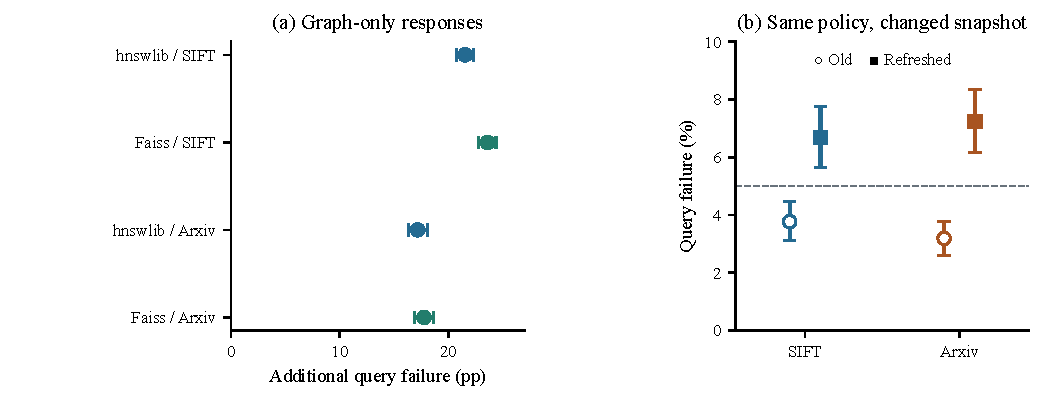
\includegraphics[width=\textwidth]{figures/overview.pdf}
\caption{Two failures that motivate ICBA. Left: graph-only transfer of retrospective first-passing actions, reported as additional failure above each target's reference. Right: one executable recurring-query policy replayed before and after a 5\% refresh. Intervals preserve shared query and target units.}
\label{fig:overview}
\Description{Four graph-only incremental-risk estimates are positive. In the refresh test, risk increases on both datasets and crosses five percent.}
\end{figure*}

\begin{table}[t]
\caption*{\textbf{Terms at a glance.} Tables shorten Arxiv-Nomic-100K to Arxiv.}
\small\begin{tabularx}{\linewidth}{@{}lX@{}}\toprule
Term & Meaning \\\midrule
ICBA & Audit contract for target portability and deployment.\\
TCP & Target-calibrated pooling for recurring profiled queries.\\
NDC & Number of distance calculations.\\
CP / UCB & Clopper--Pearson / upper confidence bound.\\
LOTO & Leave one target build out.\\
Endpoint & Largest registered native action.\\\bottomrule
\end{tabularx}
\end{table}

We make three contributions. First, we establish budget non-portability across graph-only rebuilds, data refresh, implementations, graph families, and 100K-to-1M scale while retaining each setting's estimand. Second, ICBA supplies a reusable protocol for separating response evidence, target qualification, completed execution, and information cost. Third, a preregistered recovery and baseline program identifies where complexity is warranted: target calibration is consistently valuable, TCP adds query-conditional value on SIFT, and a simple fixed action can dominate a source-tailored heuristic. The artifact independently regenerates the paper, validates the decision chain, and preserves all query-role boundaries.

The systems implication is direct: version the budget policy with its index and workload; qualify reuse on the target; and escalate from fixed to target-global to query-conditional policies only when the measured gain justifies their information cost.

\section{Related Work and Positioning}
\label{sec:related}
\sectionaim{Position the rebuild-transfer question without turning heterogeneous methods into a single leaderboard.}

\paragraph{Graph construction and maintenance.}
The final text will connect HNSW and Vamana construction choices to search-path variation. It will distinguish a rebuild of an unchanged vector collection from insert/delete-driven data refresh. Each empirical block must identify which operation it measures before these settings are discussed together.

\paragraph{Adaptive search budgets.}
DARTH, ConANN, ANNiE, and AdaEF are comparison candidates with different input signals, objectives, and execution interfaces. The literature table will record each method's published purpose, query-time information, calibration inputs, and treatment of a new build. A registered bridge is reported as that bridge, with the implementation differences stated. The present W0 numerical snapshot contains DARTH and AdaEF bridge results; it does not supply a newly verified full-method comparison for every named approach.

\paragraph{Risk control and transfer.}
The theory discussion will separate the guarantee for a fixed policy tested on independent queries from the validity of a pipeline that chooses among candidates and fallback actions. Information-theoretic limits explain why source-visible signals can be insufficient under stated observation assumptions. A measured source-to-target gap alone does not establish those assumptions.

\paragraph{Literature completion.}
This W1 section fixes the comparison axes. Bibliographic entries and detailed novelty comparisons will be imported after source and method-identity verification; no unresolved citation is represented as an established reference in this preview.

\section{Portability, Risk, and the Scope of Guarantees}
\label{sec:theory}

\subsection{Execution Risk and Retrospective Responses}
Let $G$ specify a vector snapshot, graph, and search implementation, and let $\mathcal A=(a_1<\cdots<a_J)$ be its native action grid. A policy $\pi$ maps permitted query and history observations to an action. For $q\sim\mathcal Q$,
\begin{equation}
 \begin{aligned}
 Z_G(q,a)&=\indicator\{\rec@k(G,q,a)<\tau\},\\
 \risk_G(\pi)&=\mathbb E_q Z_G(q,\pi(q)).
 \end{aligned}\label{eq:risk}
\end{equation}
Truth is computed against the corresponding snapshot. We distinguish target transport risk $\risk_{G_t}(\pi_s)$, source risk $\risk_{G_s}(\pi_s)$, and a reference-relative increment
\begin{equation}
 \Delta_{s\to t}=\risk_{G_t}(\pi_s)-\risk_{G_t}(\pi_t^{\rm ref}).\label{eq:increment}
\end{equation}
A matched old-to-new comparison instead subtracts $\risk_{G_s}(\pi_s)$, keeping the policy fixed. These two differences answer different questions.

A retrospective first-passing label is $B_G^{\rm first}(q)=\min\{a_j:Z_G(q,a_j)=0\}$. A stable-tail label is
\begin{equation}
 B_G^{\rm tail}(q)=\min\{a_j:Z_G(q,a_\ell)=0\text{ for every }\ell\ge j\}.\label{eq:stable-label}
\end{equation}
Both require query truth; an empty set is $+\infty$, an unresolved label. Native action order need not make either raw recall or realized NDC monotone. Consequently, an action larger than a first-passing label need not succeed, whereas a finite stable-tail label establishes success above it on the recorded grid. The graph-only study uses first-passing labels and evaluates the transferred action's \emph{actual} target response, rather than replacing execution failure by a budget-order comparison.

\subsection{Information Limits Explain What Must Be Observed}
\label{sec:information-limit}
The following classical two-point argument~\cite{yu1997assouad} states why source information alone may be insufficient. For two environments $E_0,E_1$, let $O$ include everything available to the decision rule, with laws $P_0^O,P_1^O$. Suppose acceptable risk--cost decisions form disjoint sets $D_0,D_1$, and loss satisfies $L_i(a)\ge\lambda\indicator\{a\notin D_i\}$ for $\lambda>0$. Then every common decision rule satisfies
\begin{equation}
 \max_i\mathbb E_i L_i(A)\ge\frac{\lambda}{2}\bigl(1-\operatorname{TV}(P_0^O,P_1^O)\bigr).\label{eq:information}
\end{equation}
Indeed, deciding whether $A\in D_0$ defines a test of the environment; its sum of error probabilities is at least $1-\operatorname{TV}$. If a common expensive endpoint is acceptable, disjointness fails and the bound can be vacuous. For random queries, $O$ must include the query jointly with its transcript. Our measurements establish response differences, not an estimate of full-observation total variation or an impossibility result for every policy. The bound explains the information question; the audit below supplies the operational test.

\subsection{Certifying a Fixed-Target Decision}
\label{sec:fixed-cert}
For a policy fixed independently of $n$ i.i.d. target-certification queries, $x$ failures yield the one-sided Clopper--Pearson bound~\cite{clopper1934confidence}
\begin{equation}
 U(x,n;\alpha)=\begin{cases}
 \operatorname{Beta}^{-1}(1-\alpha;x+1,n-x),&x<n,\\1,&x=n.
 \end{cases}\label{eq:cp}
\end{equation}
Acceptance requires $U\le\delta$. Confidence error $\alpha$ and allowed query risk $\delta$ are distinct. At zero failures, $U=1-\alpha^{1/n}$; $\alpha=\delta=0.05$ requires at least 59 queries for acceptance to be possible. With 500 certification queries, nonzero failures can be accepted, but rejection can still reflect limited power near the boundary.

\begin{proposition}[Jointly qualified selection on one target]
\label{prop:simultaneous}
Freeze $K$ policies before certification, and allocate $\alpha_j>0$ with $\sum_{j=1}^K\alpha_j\le\alpha$. On a common i.i.d. certification sample, compute $U_j=U(x_j,n;\alpha_j)$. Select any policy with $U_j\le\delta$, or abstain if none qualifies. Then
\begin{equation}
 \Pr\{\text{a policy is selected and }\risk_G(\pi_{\rm selected})>\delta\}\le\alpha.\label{eq:simultaneous}
\end{equation}
\end{proposition}
\begin{proof}
By a union bound, $\Pr\{\exists j:\risk_G(\pi_j)>U_j\}\le\sum_j\alpha_j$. Otherwise every selectable policy satisfies the risk limit. Independence among policies' bounds is unnecessary.
\end{proof}
This is simultaneous risk control~\cite{angelopoulos2021ltt}. Selection may define the policies using a separate role; the proposition then applies conditionally on selection. A fallback must be included or separately justified. The statement is per fixed target, not simultaneous over a campaign, and does not bound risk conditional on the event of acceptance. The i.i.d. query interpretation concerns the represented workload; fixed-profile replay by itself proves no guarantee for a changed query population.

\subsection{Why Pooling Is Not the Same Certificate}
\label{sec:pooling-theory}
For $m$ source builds and one target with exchangeable budget labels at a fixed query, conformal rank reasoning~\cite{angelopoulos2023conformal} gives a different guarantee. Let $r=\lceil(1-\eta)(m+1)\rceil$. Use the $r$th source order statistic if $r\le m$ and it is finite; otherwise abstain. Then
\begin{equation}
 \Pr\{a(q)<\infty,\ B_t(q)>a(q)\}\le\frac{m+1-r}{m+1}\le\eta.\label{eq:pooling}
\end{equation}
This is build-marginal label coverage for a fixed query. It translates to execution failure for stable-tail labels, but not automatically for first-passing labels. Nine sources offer rank resolution $1/10$, and old/refreshed builds need not be exchangeable. Accordingly, TCP's nine-history replay derives its target qualification from Equation~\eqref{eq:simultaneous}, not from a 5\% conformal claim. The short supplement supplies the rank proof and a margin-based selection result, and states which assumptions are uninstantiated in the experiment.

\section{ICBA and the Recovery Hierarchy}
\label{sec:auditor}

\subsection{The Audit Contract}
ICBA leaves graph construction and native traversal unchanged. Its input declares source and target snapshots, implementation, query population, action grid, permitted observations, failure event, and reference. Its output records raw reuse, candidate construction, certification counts and bounds, fallback, held-out risk, serving cost, and acquisition cost.

Selection, certification, and evaluation have disjoint roles. Selection may construct a policy. Certification checks frozen candidates and fallback; it cannot retrain or reorder them. Evaluation measures the completed decision and has no feedback path. If no action qualifies, the audit abstains. Raw reuse remains visible even when certification rejects it, so endpoint fallback cannot erase portability failure.

\subsection{A Least-Complexity Policy Ladder}
The recovery comparison is ordered by information and complexity:
\begin{enumerate}
\item a fixed native action, certified on target queries;
\item a target-global action selected and certified with target labels;
\item TCP, which retains a per-query historical profile and selects one target shift;
\item source-derived slack, retained as a portability diagnostic and ablation.
\end{enumerate}
Every candidate enters the same candidate--certificate--fallback interface. This makes a simpler passing policy evidence against the necessity of a more complex one.

\subsection{TCP: History Pooling Followed by One Target Shift}
\label{sec:tcp-implementation}
TCP uses native HNSW actions
\begin{equation}
 \mathcal A=(10,20,40,80,120,160,200).
 \label{eq:tcp-grid}
\end{equation}
For query $q$ and old build $g$, let $\tilde j_g(q)$ be the first-passing grid index, with unresolved labels retained at the endpoint. For target seed $t$, pool the nine other old builds:
\begin{equation}
 j_0^{(t)}(q)=\max_{g\in\mathcal H_t}\tilde j_g(q),\qquad
 \pi_s(q)=a_{\min\{j_0^{(t)}(q)+s,J\}}.
 \label{eq:shift}
\end{equation}
TCP applies to recurring profiled queries. Target selection scans shifts in ascending order and freezes the first shift whose selection-role CP bound passes. Candidate and endpoint then receive disjoint certification and held-out evaluation. Storing the profile costs $O(Q)$; acquisition is charged separately from serving lookup.

The original replay checks candidate and endpoint at $\alpha=.05$ each. The stricter frozen-response analysis assigns $\alpha_c=\alpha_e=.025$, applies the candidate-first order, and abstains if neither qualifies. This instantiates Proposition~\ref{prop:simultaneous} per target under its query-sampling assumptions. It is reported as a sensitivity because the confidence allocation was changed after the original replay.

\begin{figure*}[t]
\centering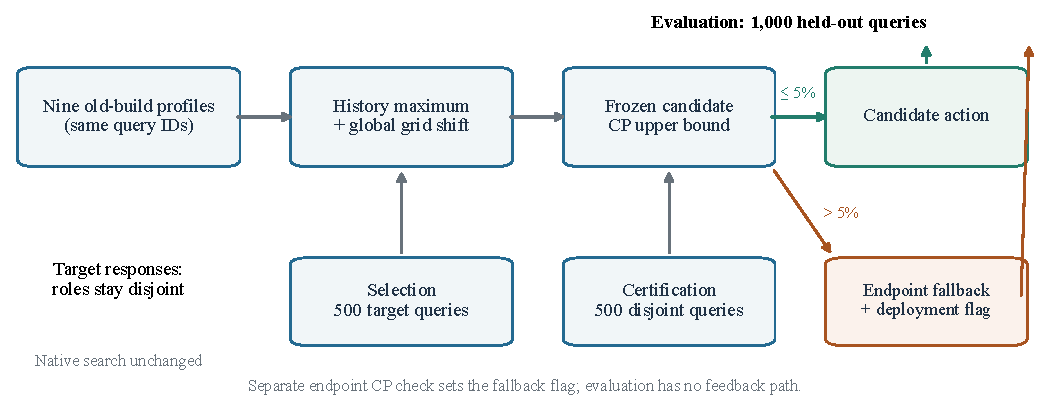
\includegraphics[width=\textwidth]{figures/workflow.pdf}
\caption{ICBA applied to a recurring-query policy. Historical profiles construct candidates; target selection freezes one rule; certification chooses candidate, endpoint, or abstention; evaluation has no feedback path. The same interface also accepts fixed and target-global candidates.}
\label{fig:workflow}
\Description{Historical response profiles feed a candidate construction stage, followed by disjoint target selection, certification, and evaluation roles.}
\end{figure*}

\subsection{Source-Derived Slack as an Ablation}
\label{sec:slack-method}
A source-design role chooses the lowest native action whose Bonferroni-adjusted CP bound passes and then shifts it upward by one grid rung, clipping at the endpoint. Later source certification and target evaluation roles are disjoint. The rule uses no target selection, so it isolates whether source evidence leaves recoverable slack. A subsequent target-certified stage freezes that candidate before new certification and evaluation roles are accessed. S9-4 compares it with fixed-256 and target-global policies on exactly the same prospective indexes and query roles. Its status is determined by that comparison, not by its absolute gain alone.

\section{Experimental Design and Inference}
\label{sec:methodology}

\paragraph{Registered settings.}
SIFT-100K uses 128-dimensional Euclidean vectors; Arxiv-Nomic-100K uses 768-dimensional normalized inner-product vectors. The graph-only study uses 24 hnswlib and 24 Faiss builds per dataset, 750 queries, and all 552 non-diagonal directions. Native grids are $(10,20,40,80,120,200)$ for hnswlib and $(16,32,64,128,256,512)$ for Faiss. Deep1M uses eight hnswlib builds and grid $(200,300,400,600,800,1200)$. Native actions are never equated across implementations.

\paragraph{Evidence stages.}
The graph-only experiment executes each source first-passing action on the target and compares it with the target first-passing reference. A separate seed-991 refresh replaces 5\% of each 100K collection, rebuilds ten old and ten refreshed indexes, and replays one recurring-query policy. TCP uses 500 selection, 500 certification, and 1,000 evaluation queries.

After these analyses were frozen, the source-slack boundary used previously untouched source-certification and target-evaluation roles. The post-seal Faiss and Deep1M studies added mutually exclusive target-certification and evaluation roles. S9-3 then created eight new insertion-permutation builds per dataset and three fresh 500-query roles, all frozen before response access. It retained the registered Faiss grid, fixed CPU, and source one-rung policy. S9-4 reused only this prospective build panel and introduced another three disjoint 500-query roles for paired baselines and ablations. Thus S9-4 is a paired method comparison, not a second independent build campaign.

\paragraph{S9-4 arms.}
The deployable arms are endpoint-512; certified fixed-256; certified source one-rung; target-global with 250 selection plus 250 certification labels; and target-global with 500 plus 500 labels. Diagnostic uncertified arms and an evaluation oracle attribute risk and headroom but cannot authorize deployment. Target-global selects the lowest estimated-cost action after removing actions whose risk UCB exceeds 5\%; failed certification executes the fixed endpoint. The 500-label arm is the equal-information comparison with the source candidate; the 1,000-label arm tests label value.

\paragraph{Metrics and timing.}
Risk is $\Pr(\rec@10<.95)$. Serving gain is $1-\bar c_{\rm policy}/\bar c_{\rm endpoint}$ for NDC or wall time, with equal query counts. We report pooled and per-target p95/p99, actual fallback, LOTO, and deletion sensitivities. Fixed-machine timing pins CPU 2, uses one search thread, 50 warmups, and seven interleaved repetitions. Top-$k$ equivalence is required before timing contributes evidence.

\paragraph{Inference.}
Primary recovery intervals use 5,000 seed-991 crossed bootstrap replicates over target builds and shared query IDs, retaining source directions within each target--query cell. Graph-only intervals resample query IDs with their complete directed-pair vectors. LOTO deletes one target without refitting. External-method and Vamana intervals retain their native units. No pooled cross-protocol effect or common leaderboard is formed.

\paragraph{Questions.}
RQ1--RQ2 establish graph-only and refresh non-portability. RQ3 tests what ICBA authorizes. RQ4 compares recovery with strong baselines. RQ5--RQ6 test tails and build sensitivity. RQ7 covers external methods, scale, and graph family. RQ8 separates measured runtime from modeled lifecycle cost. RQ9 audits reproducibility.

\section{Where Budget Portability Fails}
\label{sec:portability}

\subsection{RQ1: Do Responses Transfer When Only the Graph Changes?}
Retrospective first-passing actions frequently fail after a graph-only rebuild, even though collection membership, queries, and truth are unchanged. Table~\ref{tab:graph-only} reports absolute target risk, the unresolved-reference risk, and their difference. Across hnswlib and Faiss on both datasets, the increment ranges from 17.17 to 23.60 percentage points; every query-cluster interval is above zero. This is a response-level result independent of TCP's pooling or recalibration.

\begin{table*}[t]
\caption{Graph-only response transfer at $k=10$, $\tau=0.95$. Each row has 24 builds, 552 directed pairs, and 750 shared query IDs. Risk entries and increments are percentages or percentage points [95\% query-cluster interval], conditional on the fixed build set. The reference uses the target's own first-passing response; its failures are unresolved queries. Finite variation counts queries with at least two distinct finite first-passing actions, divided by all 750 queries.}
\label{tab:graph-only}
\small\begin{tabular*}{\textwidth}{@{\extracolsep{\fill}}llcccr@{}}\toprule
Implementation & Dataset & Absolute risk [95\% CI] & Reference risk [95\% CI] & Increment [95\% CI] & Finite variation\\\midrule
\GraphOnlyRows
\bottomrule\end{tabular*}
\end{table*}

The variation is principally among finite budgets: 75.87--91.07\% of queries have different finite first-passing actions across builds, while only 0.53--2.67\% switch between resolved and unresolved states. Removing the 1\% of queries with largest incremental contribution leaves increments of 21.37/16.95 percentage points for hnswlib and 23.43/17.53 for Faiss, on SIFT/Arxiv respectively. Endpoint censoring and a handful of extreme queries therefore do not explain the result.

This experiment diagnoses the budget--response relation using retrospective truth on both source and target. It establishes that source success alone is insufficient evidence for action reuse. The measured mechanism is behavioral variation across builds; structural attribution to particular edges or navigation paths lies outside this response-level design.

\subsection{RQ2: Does an Executable Policy Deteriorate after Refresh?}
The matched old/new replay holds the nine-history policy fixed and applies it to both snapshots. Unlike RQ1, this changes 5\% of the vectors as well as rebuilding. SIFT's empirical risk rises from 3.77\% to 6.69\%; Arxiv-Nomic's rises from 3.19\% to 7.24\%. The corresponding paired increments [crossed 95\% interval] are 2.92 [1.75, 4.07] and 4.05 [2.86, 5.31] percentage points. Thus this is a measured deterioration, not merely an absolute target risk with an unknown source baseline.

Independent single-policy CP checks at $\alpha=0.05$ qualify six of ten old SIFT policies and five of ten old Arxiv policies. All eleven fail the corresponding target check. This paired diagnostic uses per-policy checks rather than simultaneous control over the eleven transitions. Target evaluation risk exceeds 5\% in all ten builds of each dataset; removing the highest-risk target leaves 6.61\% and 7.13\%. The deterioration is distributed across targets.

The same policy information is held fixed in each old/new comparison, but the experiment does not separate changed graph paths from changed nearest-neighbor membership. Together, RQ1 and RQ2 establish complementary facts: unchanged data do not make the response function portable, and a recurring-query policy can lose its old qualification after refresh plus rebuilding.

\section{Audit Decisions, Recovery, and Strong Baselines}
\label{sec:recovery-results}

\subsection{RQ3: What Does ICBA Authorize?}
Direct unshifted reuse fails every candidate certificate in the original refresh replay and routes all 20 targets to the endpoint. ICBA therefore blocks unsafe efficiency without manufacturing a saving. TCP changes the candidate before certification. The original allocation accepts 19/20 candidates; the $.025+.025$ sensitivity accepts all ten SIFT and six Arxiv candidates, with four certified endpoint fallbacks and no abstention.

\begin{figure*}[t]
\centering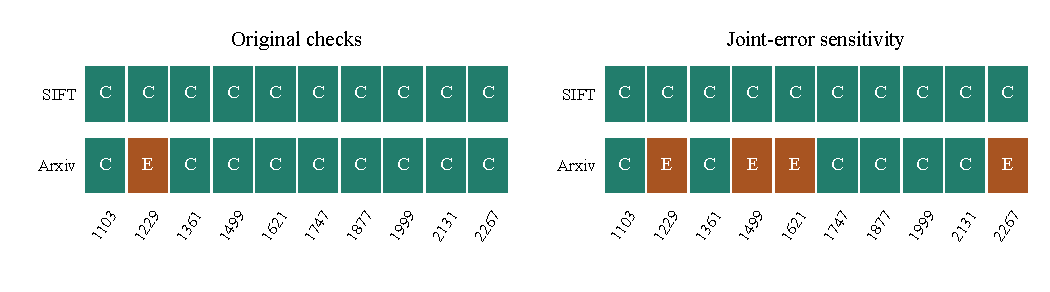
\includegraphics[width=\textwidth]{figures/decisions.pdf}
\caption{Completed target decisions. C denotes candidate and E endpoint fallback. The stricter $.025+.025$ allocation changes Arxiv composition from nine to six candidates while every completed decision remains qualified.}
\label{fig:decisions}
\Description{SIFT accepts ten candidates under both rules. Arxiv accepts nine under the original allocation and six under the stricter allocation.}
\end{figure*}

\subsection{RQ4: Endpoint-Relative Recovery and Incremental Value}
TCP's original completed decisions reduce mean NDC by 44.39\% on SIFT and 44.79\% on Arxiv. Under the joint-error allocation, SIFT is unchanged and Arxiv retains 29.86 [14.75,45.00]\%. Risk is 1.79\% and 1.68\%, respectively. Both remain positive relative to each target's endpoint.

The equal-information comparison asks the stronger question. Against target-global calibration with the same 500 selection, 500 certification, and 1,000 evaluation queries, TCP gains a further 27.60 [17.92,36.72]\% mean NDC on SIFT, but Arxiv's 10.78\% interval includes zero and its p95 ratio is 1.109. Query conditioning therefore adds resolved value only on SIFT under the registered event, grid, and SLA.

\begin{figure}[t]
\centering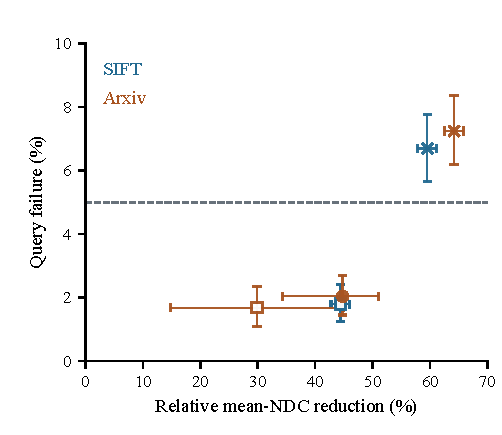
\includegraphics[width=\linewidth]{figures/tradeoff.pdf}
\caption{Refresh risk--work tradeoff with crossed 95\% intervals. Direct reuse is efficient but crosses the risk target; certification and fallback move completed decisions toward the endpoint.}
\label{fig:tradeoff}
\Description{Direct reuse has high failure. Target-recalibrated policies have lower risk and retain positive search-work savings.}
\end{figure}

\subsection{Prospective Fresh-Build Confirmation}
\label{sec:prospective}
\label{sec:fresh-bridge}
S9-3 freezes a one-rung candidate before eight new insertion-permutation builds and three fresh query roles per dataset are accessed. All 56 directed decisions per dataset accept the candidate, with zero fallback or abstention (Table~\ref{tab:s9-prospective}). Across 144,000 response cells and 112,000 raw timing measurements, native and measured top-$k$ agree exactly. Sparse-grid and 2.5\%-risk sensitivities remain safe but collapse to the endpoint, defining preregistered boundaries rather than failures of the primary configuration.

\begin{table*}[t]
\caption{S9-3 prospective confirmation on eight new target builds per dataset. Risk and wall-time reduction are percentages [95\% crossed target-build/query interval]. P95 is the policy/endpoint wall-time ratio [95\% interval]; LOTO is minimum wall-time reduction after deleting one target.}
\label{tab:s9-prospective}
\small\begin{tabular*}{\textwidth}{@{\extracolsep{\fill}}lrrrr@{}}\toprule
Dataset & Eval. risk & Wall-time reduction & P95 ratio & LOTO reduction\\\midrule
\SProspectiveRows
\bottomrule\end{tabular*}
\end{table*}

\subsection{Strong Baselines Change the Method Conclusion}
S9-4 evaluates fixed and target-calibrated policies on the same prospective indexes with new disjoint roles (Table~\ref{tab:s9-baselines}). Every deployable arm passes risk, mean-wall, p95, LOTO, and timing-stability gates. Fixed-256 exactly matches source one-rung on SIFT and exceeds it by 10.91 wall-time percentage points on Arxiv. The source heuristic is therefore unnecessary on this panel.

The equal-information target-global-500 arm remains safe and positive but falls back on 7/56 decisions per dataset, widening its interval. With 500 selection plus 500 certification labels, target-global-1000 is strongest on both datasets. This is a label-value result, not an equal-information victory. The evaluation oracle leaves additional SIFT headroom; on Arxiv, the label-rich target arm reaches the oracle action pattern.

\begin{table*}[t]
\caption{S9-4 paired strong-baseline audit. Risk and wall-time reduction are percentages [95\% crossed interval]. P95 gives ratio (95\% upper bound); LOTO is minimum reduction. Target-global-500 uses 500 labels total, target-global-1000 uses 1,000.}
\label{tab:s9-baselines}
\small\begin{tabular*}{\textwidth}{@{\extracolsep{\fill}}llrrrr@{}}\toprule
Dataset & Candidate & Risk & Wall-time reduction & P95 ratio & LOTO\\\midrule
\SStrongBaselineRows
\bottomrule\end{tabular*}
\end{table*}

\paragraph{Mechanism attribution.}
Moving one rung above the source action lowers held-out risk from 2.15\% to 0.40\% on SIFT and from 1.775\% to 0.307\% on Arxiv, while sacrificing 24.92 and 31.21 NDC-gain points. Certification changes authorization but not execution when every candidate passes. Target labels, rather than source-specific tailoring, drive the largest additional gains.

\subsection{RQ5--RQ6: Tail and Build Stability}
For historical joint-error TCP, pooled p95/p99 remain below the endpoint and every target has non-increasing tails. S9-3 and S9-4 also pass p95 and LOTO gates; the least favorable S9-4 p95 upper bound is 0.930 for SIFT target-global-500 and 0.921 for its Arxiv counterpart. The prospective conclusions therefore do not depend on one target build, although eight builds remain an underpowered basis for open-population inference.

\section{RQ7: Scope across Methods, Scale, and Graph Family}
\label{sec:families}

\paragraph{External adaptive methods.}
The frozen DARTH adapters produce target query-failure rates of 22.55\% on SIFT-100K and 23.12\% on Arxiv-Nomic-100K at $\rec@10<0.95$. Ada-ef yields 9.52 [9.44, 9.60]\% on ten Arxiv targets, with a target-build bootstrap conditional on its query set. All ten Ada-ef candidate certificates fail; audited execution uses the qualified endpoint and has zero search gain relative to that endpoint. Ada-ef is absent from Euclidean SIFT because the inspected estimator implements cosine/inner-product semantics, not a semantics-preserving L2 path. Its exclusion is an implementation-scope boundary, not a failed SIFT result.

These measurements show why query-risk qualification matters beyond TCP. They do not, without matched source checks, identify how much failure was caused by rebuilding, and the event is not interchangeable with mean recall or expected false-negative fraction. They therefore remain qualification studies rather than a ranking of published methods. The TCP comparator and information budget are stated separately.

\paragraph{Larger scale.}
On Deep1M, eight hnswlib builds cross four seeds with two insertion orders, giving 56 directed pairs on 1,000 queries. Source-derived first-passing actions have 28.86\% transport risk against 8.82\% target-reference risk. The incremental risk is 20.04 [17.29, 22.77] percentage points, using a target-build bootstrap conditional on the frozen source histories and query set. Keeping the reference risk visible matters: this is additional loss above a difficult, partly unresolved target reference, not a transfer from a zero-risk baseline.

A preregistered replication reuses the eight indexes with disjoint 500/500/500-query roles. All 56 non-clipped candidates pass target certification; evaluation risk is 1.63 [0.80, 2.61]\% and mean-NDC saving versus efSearch 1200 is 34.28 [33.53, 35.05]\%. Every target and leave-one-target-out analysis remains positive; this is scale, not cross-family, confirmation.

\paragraph{Vamana-style evidence.}
Six source and six separate target builds produce 36 directions and 750 queries per dataset, using native search-list size and beam width one. The frozen event table combines its stage-specific under-budget and censoring outcomes. A target-build reanalysis gives 16.86 [15.88, 17.93]\% on SIFT and 11.37 [10.80, 11.99]\% on Arxiv. Its recorded responses do not reconstruct exactly the first-passing execution estimand used for hnswlib/Faiss. We retain it as directional cross-family evidence, not another row of Table~\ref{tab:graph-only}.

Vamana cost-tax intervals include zero: 1.07 [$-1.03$, 2.86]\% and 1.17 [$-0.83$, 3.03]\%, respectively, for the mean of per-target ratios in that reanalysis. Thus it supplies no established positive cost penalty or cross-engine superiority. Table~\ref{tab:scope} summarizes which question each setting can answer.

\begin{table*}[t]
\caption{Scope of the extension evidence. Each row retains its event, reference, and inference unit. All numeric intervals in the text are 95\%; no common cross-engine ranking or pooled effect is formed.}
\label{tab:scope}
\small\begin{tabularx}{\textwidth}{@{}lXXl@{}}\toprule
Setting & Event and reference & Supported comparison & Unit / query count\\\midrule
DARTH & Absolute target $\rec@10<0.95$ risk; no matched reference subtraction & Target qualification under the frozen adapter & Target summaries; 1,000/build\\
Ada-ef & Absolute target $\rec@10<0.95$ risk; endpoint for audited saving & Candidate rejection versus endpoint execution on Arxiv & 10 target builds; 1,000/build\\
Deep1M & Transport versus target reference; certified slack versus efSearch 1200 & Transfer loss and certified recovery at 1M scale & 8 targets; 1,000 prior + 1,500 fresh\\
Vamana-style & Frozen stage under-budget/censoring event; stage-specific cost reference & Directional cross-family transfer evidence, not a harmonized HNSW increment & 6 target builds; 750 shared queries\\\bottomrule
\end{tabularx}
\end{table*}

Together with RQ1, these results support a layered conclusion: response non-portability is seen across HNSW implementations and at larger scale; qualification of adaptive actions is operationally consequential; and a distinct graph family supplies supporting evidence with narrower semantic comparability. They do not establish uniform failure across every graph family or every adaptive policy.

\section{RQ8: Runtime and Lifecycle Value}
\label{sec:recovery}

NDC is implementation-independent search work; elapsed time is the deployment endpoint. We therefore report both without substituting one for the other.

\paragraph{Measured fixed-machine runtime.}
The S9-2 timing campaign pins one CPU, one search thread, and interleaves seven repetitions after 50 warmups over 24 builds per dataset. The original sub-millisecond per-cell CV criterion was rejected before policy gains were inspected; an amended action-block stability gate passes with exact native equivalence. The frozen source-slack candidate reduces wall time by 9.44 [9.04,9.77]\% on SIFT and 26.04 [25.62,26.44]\% on Arxiv. P95 ratios are 0.988 and 0.914, and minimum LOTO reductions are 9.42\% and 25.97\%. S9-3 and S9-4 independently retain positive fixed-machine wall-time reductions on fresh roles and builds.

\paragraph{Lifecycle accounting.}
For policy $\pi$ at horizon $N$,
\begin{equation}
 C_\pi(N)=C_{{\rm acquire},\pi}+N\bar c_\pi,
 \qquad N_{\rm BE}=\frac{\Delta C_{\rm acquire}}{\bar c_{\rm end}-\bar c_\pi}.
 \label{eq:breakeven}
\end{equation}
Cached history treats old profiles and truth as sunk; cold history charges their acquisition once per snapshot. Target selection, candidate and endpoint certification, and exact target truth are charged to recovery. At $N=10^6$, cold-history joint-error TCP saves about 490 million NDC on SIFT and 389 million on Arxiv; break-even is approximately 396,000 and 457,000 executions, compared with 129,000 and 148,000 under cached history. Four Arxiv fallback targets do not individually amortize positive recovery overhead.

\begin{table}[t]
\caption{Joint-error TCP break-even executions in thousands [95\% target-build interval]. ``No saving'' counts nonamortizing targets.}
\label{tab:economics}
\small\begin{tabular*}{\linewidth}{@{\extracolsep{\fill}}llrr@{}}\toprule
Dataset & History & Break-even, $10^3$ & No saving\\\midrule
\CostRows
\bottomrule\end{tabular*}
\end{table}

The post-seal target-certified Faiss ledger charges one 500-query target audit per target and reuses it across 23 source histories. Portfolio break-even is 66,914/17,018 executions under pairwise accounting and 3,019/755 under shared-target accounting for SIFT/Arxiv. These are NDC ledgers. Historical source acquisition and exact-truth/control wall time are unavailable and are not assigned zero. The measured S9 timing results establish serving latency reduction on one machine; they do not convert the NDC lifecycle model into a hardware-general monetary claim.

\begin{figure}[t]
\centering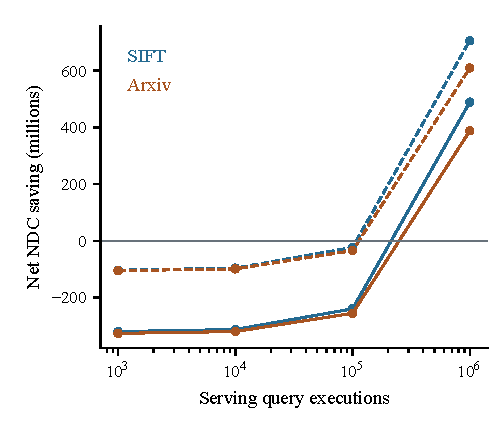
\includegraphics[width=\linewidth]{figures/cost.pdf}
\caption{Modeled joint-error TCP net distance saving versus serving horizon. Cold history crosses zero later than cached history; fallback targets remain in the average.}
\label{fig:cost}
\Description{Net distance savings become positive only after the acquisition cost is amortized over a sufficiently long serving horizon.}
\end{figure}

\section{Reproducibility, Scope, and Operational Rule}
\label{sec:discussion}

\subsection{RQ9: Can the Decision Chain Be Replayed?}
The anonymous package contains 107 files and no identity leaks. A clean environment imports no main-repository code, rebuilds the paper and supplement, regenerates six figures and five data-linked tables, and passes 244 baseline checks, 1,205 post-seal checks, and 210/210 source-policy checks. A fresh Faiss environment reproduces registered native action rows with zero top-$k$, recall, NDC, or action-order mismatch. S9-3 adds 144,000 response cells, 112,000 timing measurements, and 16,000 top-$k$ checks with zero mismatch. S9-4 adds another 144,000 response cells and 20,500 checks, again with zero mismatch. Role manifests retain zero overlap among selection, certification, and evaluation.

The latest S9 records are committed with checksums and deterministic regeneration scripts. The procedural consistency audit follows a local scientific-writing checklist~\cite{kassis2026scientific}; all numeric claims remain bound to repository records rather than generated prose.

\subsection{What the Evidence Establishes}
Budget response changes across registered graph rebuilds, data refresh, implementations, and scale. ICBA detects this change and converts a frozen candidate into a target-qualified completed decision. TCP recovers endpoint-relative work for recurring profiled queries and adds resolved value beyond target-global calibration on SIFT. Target-global calibration is the stronger default on Arxiv. Source-derived slack can work, but S9-4 shows that a fixed action can match or dominate it.

The resulting maintenance rule has three steps. First, audit inherited policies against the target event and endpoint. Second, certify the least complex viable candidate and its fallback on disjoint target queries. Third, escalate from fixed to target-global to query-conditional policies only when held-out gain and lifecycle accounting justify the additional information.

\subsection{Boundaries}
The main conclusions are conditional on registered query populations, grids, SLAs, and build panels. The prospective S9 panel has eight builds per dataset and one CPU configuration; S9-4 reuses that build panel for paired attribution. TCP assumes recurring profiled queries. The complete cold-history ledger is expressed in NDC, while actual timing covers serving search rather than truth acquisition, control, energy, or storage. DARTH, Ada-ef, Deep1M, and Vamana retain different native estimands and support scope rather than a common ranking. These boundaries define the next replication targets without changing the fixed-target decisions reported here.

\section{Conclusion}
Search-budget portability is an index-conditioned deployment decision. ICBA makes that decision auditable by separating candidate construction, target certification, fallback, held-out evaluation, and cost. The evidence rejects automatic reuse, confirms safe recovery on fresh builds and queries, and shows why strong simple baselines are essential: fixed-256 can dominate source-tailored slack, while target calibration provides the largest robust gains and TCP is valuable when recurring query histories add measurable information. The practical outcome is a complexity-aware policy ladder backed by target evidence rather than a universal recovery rule.

\balance
\bibliographystyle{ACM-Reference-Format}
\bibliography{references}
\end{document}
